\documentclass[11pt]{article}

\usepackage[margin=0.82in]{geometry}
\usepackage{amsmath,amssymb,mathtools}
\usepackage{booktabs,tabularx,array}
\usepackage{graphicx,subcaption,float,placeins}
\usepackage{enumitem}
\usepackage{microtype}
\usepackage{xcolor}
\usepackage{hyperref}

\hypersetup{
  colorlinks=true,
  linkcolor=blue!45!black,
  urlcolor=blue!55!black,
}

\newcommand{\norm}[1]{\left\lVert #1\right\rVert}
\newcommand{\inner}[2]{\left\langle #1,#2\right\rangle}
\newcommand{\eref}{e_\eta}
\newcommand{\eshift}{e_{\eta,\mathrm{shift}}}
\allowdisplaybreaks

\title{Weekly Presentation: Learned Dirichlet--Neumann Rollouts\\
Experiments and Results from 9--16 July 2026}
\author{Internal project summary}
\date{16 July 2026\\Data cutoff: 05:30 EDT}

\begin{document}
\maketitle

\section*{Summary}

The project began the week with occasional learned rollouts that amplified
intermediate and high Fourier modes until a Gauss--Legendre stage calculation
became nonfinite.  Direct spectral damping and smaller time steps changed when
failure occurred but did not remove it.  The important observation was that
the learned DNO could have small value error on a reference trajectory while
having a badly wrong derivative with respect to the surface shape $\eta$.

This motivated model C16: evaluate $G_0+G_1$ from their formulas, learn only an
$O(\eta^2)$ self-adjoint remainder, penalize violation of the Hadamard shape
derivative, and evaluate the quadratic Zakharov terms with twofold Fourier
dealiasing.  These changes were made together.  The resulting fixed 320-case
test had no observed nonfinite model trajectory.  The experiment supports the
complete bundle; it does not identify which ingredient was individually
necessary.

The present checkpoint, C21, was tested on 2,560 newly generated initial
conditions.  The order-six numerical reference was valid in 2,508 cases.  C21
was finite in all 2,508.  Its median terminal relative elevation error is
$.00563$ and its 95th percentile is $.1693$, but six finite cases have error
above one.  Five are Tanaka cases whose error is mostly horizontal displacement.
The sixth is a Benjamin--Feir case with incorrect Fourier-mode amplitudes and
phases; it cannot be repaired by one horizontal shift.

C25 is now testing a simple hypothesis: perhaps the constrained neural
remainder is too small.  Relative to C20, C25 keeps the equations, exact
$G_0+G_1$ terms, neural construction, data, and loss fixed, and increases the
parameter count from 860,928 to 1,342,400.  It is a fresh retraining, not
another phase-specific loss experiment.  Four epochs are complete and epoch 5
is in progress at the stated cutoff.  There is no C25 rollout result yet.

\section{The numerical comparison}

Let $z=(\eta,\xi)$, where $\eta$ is surface elevation and $\xi$ is surface
potential.  The DNO supplies
\begin{equation}
  q=G(\eta;h)\xi=\eta_t.
  \label{eq:q}
\end{equation}
With gravity normalized to one, the equations used in the code are
\begin{align}
  \eta_t&=q,\\
  \xi_t&=-\eta-\frac12\xi_x^2
  +\frac12\frac{(q+\eta_x\xi_x)^2}{1+\eta_x^2}.
  \label{eq:zakharov}
\end{align}
The learned and reference rollouts use the same $1024$-point periodic grid,
inner step $.01$, two-stage Gauss--Legendre integrating-factor method, four
Picard iterations, and fixed projection onto $|k|\leq128$.  The numerical
reference uses a Craig--Sulem series through $G_6$ with eightfold padding.  It
is a numerical reference, not the exact continuum solution.  The learned
calculation replaces only the evaluation of $q$.

If $\Phi_6$ and $\Phi_\theta$ denote one complete numerical step with the
reference and learned DNOs, respectively, then
\begin{equation}
\begin{split}
z_{n+1}^\theta-z_{n+1}^6
={}&\underbrace{\Phi_\theta(z_n^\theta)-\Phi_6(z_n^\theta)}_{
\text{error caused by replacing the DNO at the current model state}}\\
&+\underbrace{\Phi_6(z_n^\theta)-\Phi_6(z_n^6)}_{
\text{propagation of state error already present}}.
\end{split}
\label{eq:split}
\end{equation}
This exact identity organizes the experiments.  Pointwise training acts on the
first term at sampled states.  Long rollouts also depend on how earlier errors
move the state and are subsequently propagated by the second term.

\section{Why the Hadamard shape derivative mattered}

\subsection{The evidence before changing the architecture}

The old failures looked spectral at the end, but the following measurements
showed that the error began earlier in the learned operator.

\begin{itemize}[leftmargin=*]
  \item At selected reference states preceding failure, the relative error in
  $q$ was only about $1.7$--$1.9\times10^{-4}$.

  \item A small displacement in the direction actually produced by the model
  changed the learned $q$ with a finite secant gain of about $8.1$--$8.4$.
  The displacement-induced output change was $2.4$--$2.6\times10^4$ times the
  original value error on the reference state.

  \item A perturbation at Fourier mode 117 produced an erroneous learned
  response at mode 115 of about $985.7$, compared with
  $1.47\times10^{-5}$ for the order-six reference.

  \item Twofold dealiasing of the nonlinear right-hand side delayed three
  failures by only $.05$, $.08$, and $.05$ time units.  It did not remove the
  preceding operator error.
\end{itemize}

The first two Craig--Sulem terms are
\begin{align}
  \widehat{G_0(h)\xi}_k
  &=|k|\tanh(h|k|)\widehat\xi_k,\\
  G_1(\eta;h)\xi
  &=-G_0\bigl(\eta G_0\xi\bigr)
    -\partial_x\bigl(\eta\partial_x\xi\bigr).
  \label{eq:g1}
\end{align}
The two terms in $G_1$ provide a cancellation for the same-sign interaction
detected above.  Hard-coding $G_1$ prevents the network from approximating two
large terms separately and missing their small difference.

\subsection{The shape identity}

For any perturbation $\zeta$ of the surface, the DNO satisfies
\begin{equation}
  D_\eta G(\eta)[\zeta]\xi
  +G(\eta)(\zeta B)+\partial_x(\zeta V)=0,
  \label{eq:hadamard}
\end{equation}
where
\begin{equation}
  B=\frac{G(\eta)\xi+\eta_x\xi_x}{1+\eta_x^2},
  \qquad
  V=\xi_x-B\eta_x.
  \label{eq:BV}
\end{equation}
This identity constrains the derivative with respect to $\eta$, not merely the
value $G(\eta)\xi$.  On three examined states, the old model's relative
residual in \eqref{eq:hadamard} was $1.394$, $.502$, and $2.724$.  The
order-six reference gave $1.43\times10^{-5}$,
$3.43\times10^{-6}$, and $3.82\times10^{-6}$ in the same discrete test.

The training loss uses a finite secant
\begin{equation}
  S_\varepsilon
  =\frac{G_\theta(\eta+\varepsilon\zeta)\xi
  -G_\theta(\eta)\xi}{\varepsilon}
\end{equation}
and penalizes the relative $H^1$ energy of
\begin{equation}
  S_\varepsilon
  +G_\theta(\eta)(\zeta B_\theta)
  +\partial_x(\zeta V_\theta).
  \label{eq:had-loss-short}
\end{equation}
The random direction $\zeta$ is spectrally smoothed and restricted to
$0<|k|\leq128$; $\varepsilon$ is sampled between $10^{-3}$ and
$3\times10^{-3}$.  The loss is evaluated on a small batch once every 16
optimizer steps.  It enforces self-consistency of the learned derivative; the
ordinary supervised loss is still needed to anchor the value of the operator.

\subsection{What C16 changed and what the result means}

C16 combined five changes:
\begin{enumerate}[leftmargin=*]
  \item explicit, uncut evaluation of $G_0+G_1$;
  \item a learned correction beginning at $O(\eta^2)$;
  \item self-adjointness in $\xi$ from tied real Fourier multipliers;
  \item the randomized finite-secant loss \eqref{eq:had-loss-short}; and
  \item twofold dealiasing in the quadratic equation for $\xi_t$.
\end{enumerate}
C16 produced no nonfinite model trajectory in the fixed 320-case test without
runtime damping or an output cap.  Two Tanaka cases still had finite terminal
error above one.  The justified conclusion is that the bundle removed the
observed nonfinite behavior on this sample.  There was no full factorial
ablation, so the experiment does not identify one individually sufficient
ingredient.

\begin{figure}[htbp]
  \centering
  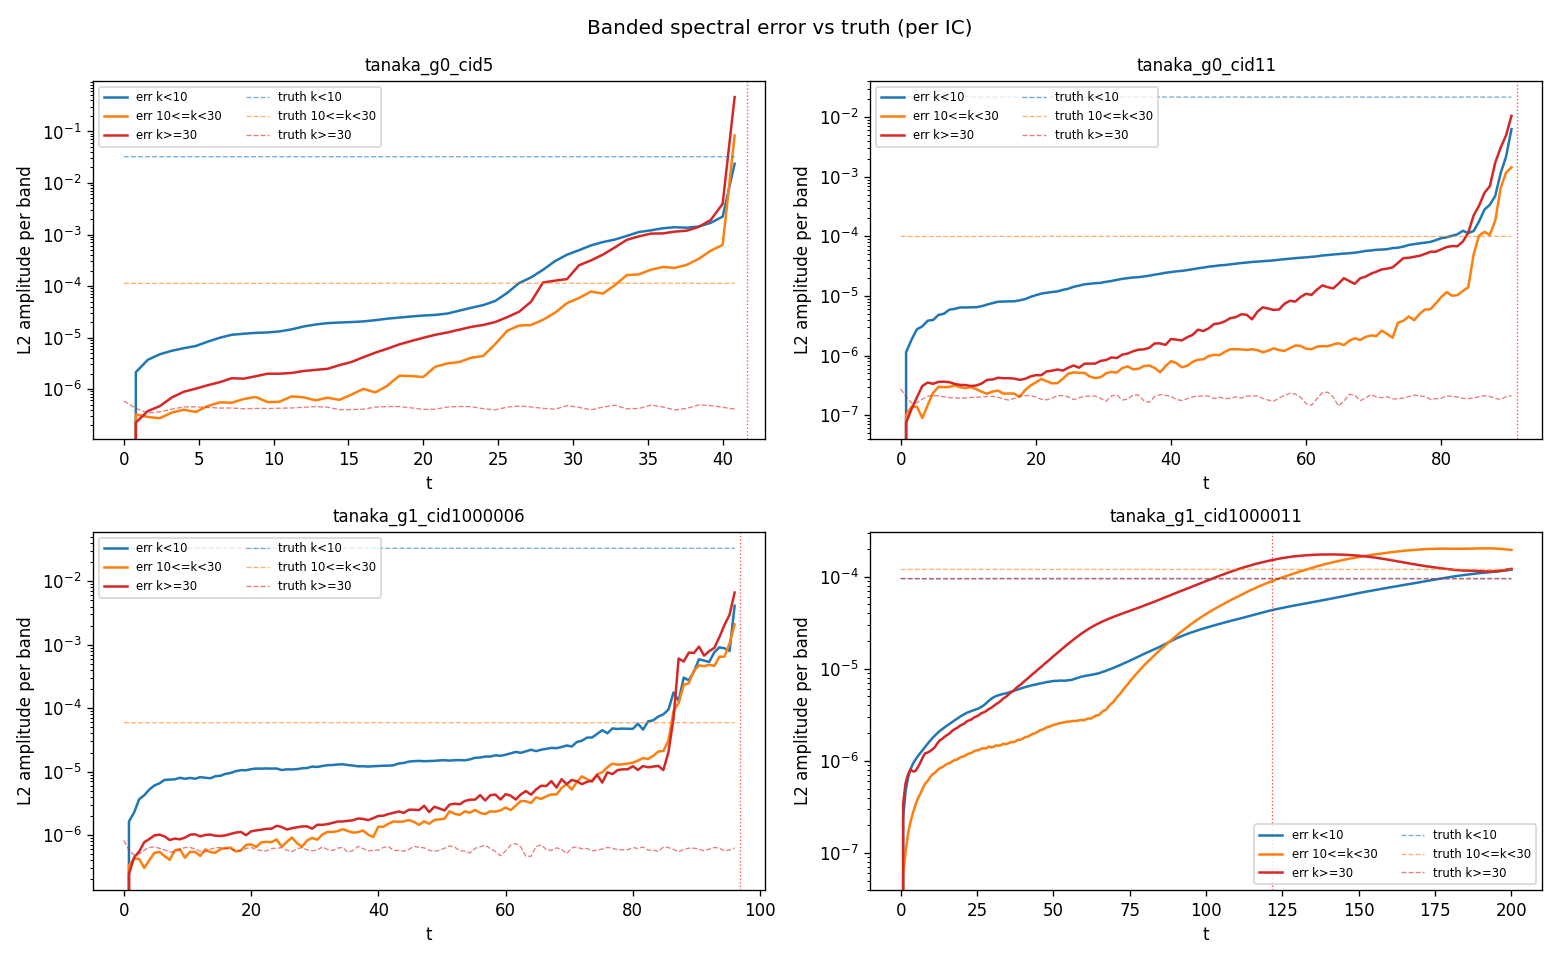
\includegraphics[width=\textwidth]{../figures/tanaka_audit/banded_spectral.png}
  \caption{Fourier-band error in representative models before C16.  This is
  the behavior that made high-frequency penalties and damping reasonable to
  test.  Those methods acted on the visible late symptom; the derivative tests
  identified an earlier learned-DNO error.}
  \label{fig:old-growth}
\end{figure}

\FloatBarrier

\section{The experiments that followed}

The following table keeps only the experiments needed to understand the
current model.  Counts refer to the stated fixed comparison panels and should
not be read as population probabilities.

\begin{table}[htbp]
\centering
\small
\begin{tabularx}{\textwidth}{p{.09\textwidth}p{.24\textwidth}X p{.22\textwidth}}
\toprule
Run & Question & Result & What we retained \\
\midrule
C8--C10
& Can a penalty on the growing Fourier band prevent the old NaNs?
& The best version reduced Tanaka nonfinite cases from 3/32 to 2/32 but
increased finite errors.  Runtime limiting did not remove the remaining two.
& Spectral growth is a useful warning signal, not a sufficient training target. \\

C14
& Can the high-frequency output be bounded by architecture?
& The best finite checkpoint retained 3/32 nonfinite Tanaka trajectories and
training became nonfinite after epoch 25.
& Do not use the tested output bound. \\

C16
& Does the $G_0+G_1+O(\eta^2)$, self-adjoint, Hadamard-regularized construction
remove the observed nonfinite behavior?
& No nonfinite model trajectory in the fixed 320-case test; remaining large
errors were finite Tanaka errors.
& This is the model construction used afterward. \\

C19
& Does a Gaussian-localized translation-speed loss prevent cancellation
between separated crests?
& Several multi-crest Tanaka cases improved, but some BF and linear upper
quantiles increased.
& Retain it as one part of the objective, not as a complete error model. \\

C20
& Does a fresh retraining that also gives weak active Fourier modes more
influence improve Tanaka and Benjamin--Feir errors?
& No nonfinite model trajectory in the fixed 320 cases; aggregate Tanaka and
selected BF errors improved; one finite translated Tanaka case exceeded one.
& This is the loss used for the present full retraining. \\

C21
& Was C20's localized tangent coefficient too small?
& One low-learning-rate epoch with coefficient 100 improved the fixed aggregate
and case 27, but worsened the two-crest case 24.
& Use C21 for current evaluation; do not regard weight 100 as a universal fix. \\

C22
& Does weighting local speed error by instantaneous relative elevation
sensitivity improve the shallow, narrow profiles?
& Case 27 improved; case 24 and the aggregate did not beat C21.
& The sensitivity is informative, but the tested loss is not the next model. \\

C23
& Can a sparse eight-step full-state loss replace C21's dense tangent term?
& The result returned close to C20.  The new term covered only $.08$ time units
and contributed about $.177\%$ after its once-per-16 schedule.
& The tested sparse configuration was too weak; it does not rule out all
finite-time training. \\
\bottomrule
\end{tabularx}
\caption{The main experiments from 9--15 July and the limited conclusions they
support.}
\label{tab:experiments}
\end{table}

\section{What C21 currently achieves}

\subsection{Evaluation set and error definition}

There are ten named panels but seven physical initial-condition distributions:
two independent Tanaka panels, three independent Benjamin--Feir panels, a
linear single-mode panel, deep and finite-depth random seas, and deep and
finite-depth Stokes panels.  Each named panel contains 256 independently
generated initial conditions.  Long Tanaka and Benjamin--Feir rollouts end at
$T=200$; the other panels end at $T=20$.

A reference is valid if all saved $(\eta,\xi,q)$ values are finite and its
maximum relative Hamiltonian drift is at most $10^{-3}$.  Of 2,560 attempted
references, 2,508 are valid.  C21 has no saved nonfinite value on these 2,508
cases.

The primary terminal error is
\begin{equation}
  \eref(T)=
  \frac{\norm{\eta^\theta(T)-\eta^6(T)}_2}
       {\norm{\eta^6(T)}_2}.
  \label{eq:raw}
\end{equation}
For diagnosis, we also numerically minimize over one periodic translation:
\begin{equation}
  \eshift(T)=\min_s
  \frac{\norm{\eta^\theta(\cdot-s,T)-\eta^6(\cdot,T)}_2}
       {\norm{\eta^6(T)}_2}.
  \label{eq:shift}
\end{equation}
The raw error remains the model-comparison metric.  The shifted error measures
how much of the final discrepancy is explained by horizontal position.

\begin{table}[htbp]
\centering
\small
\begin{tabular}{lrrrrrrrr}
\toprule
Error & Median & $q_{75}$ & $q_{90}$ & $q_{95}$ & $q_{99}$ & Max & Count $>.25$ & Count $>1$ \\
\midrule
Raw & .005634 & .020413 & .083930 & .169262 & .485363 & 1.326217 & 83 & 6 \\
After one shift & .003709 & .011708 & .032467 & .058772 & .207540 & .842246 & 17 & 0 \\
\bottomrule
\end{tabular}
\caption{C21 terminal relative elevation error on the 2,508 valid references.
There are also 23 raw errors above .50 and 11 above .75; after one shift these
counts are 5 and 1.}
\label{tab:c21-summary}
\end{table}

\begin{figure}[htbp]
  \centering
  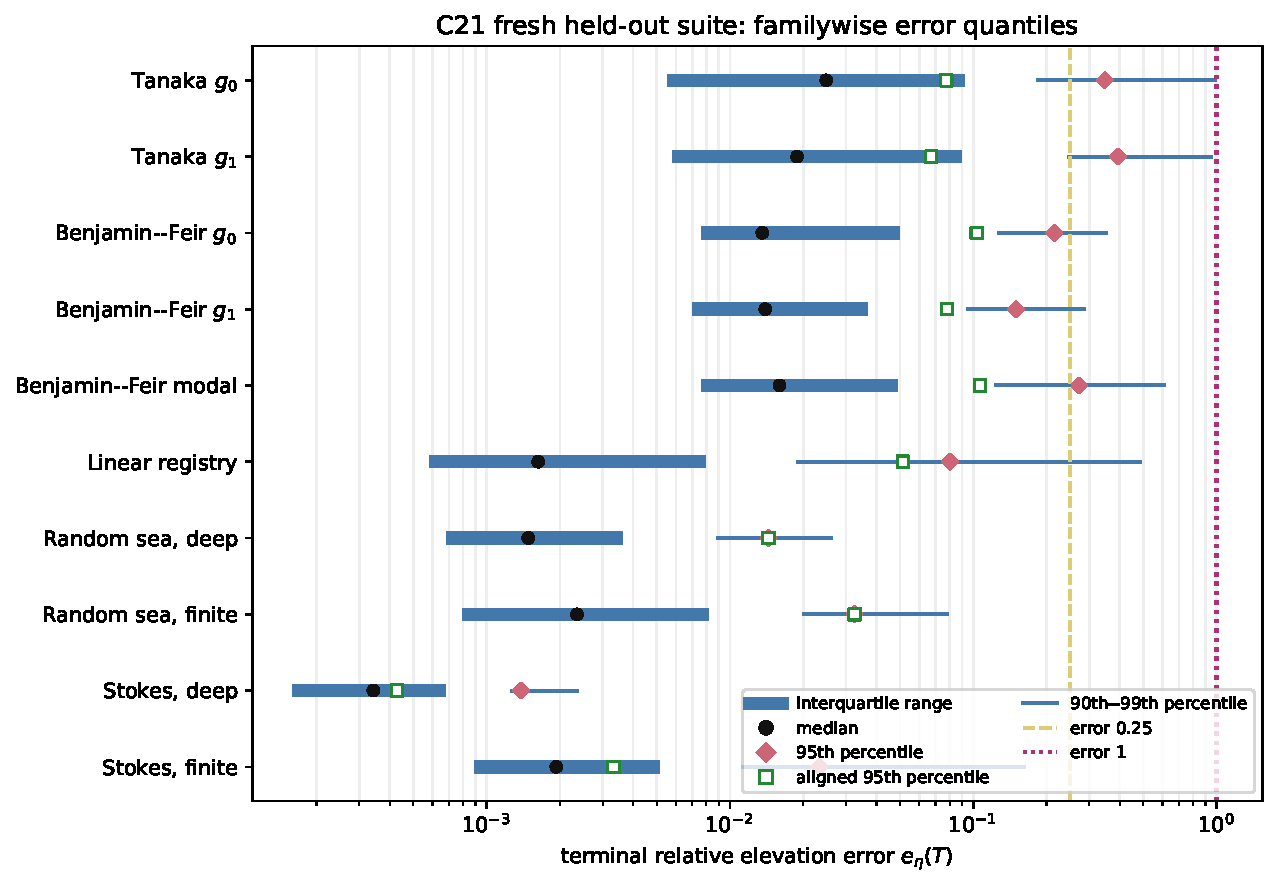
\includegraphics[width=\textwidth]{../figures/weekly_results_20260716/c21_heldout_family_quantiles.pdf}
  \caption{C21 empirical error quantiles separated by initial-condition panel.
  Black circles are raw medians, red diamonds are raw 95th percentiles, and
  open green squares are 95th percentiles after one horizontal translation.}
  \label{fig:quantiles}
\end{figure}

\FloatBarrier

\section{What we are trying to solve now}

\subsection{Tanaka: gradual horizontal displacement}

Five of the six raw errors above one are Tanaka cases.  Their raw and shifted
errors are
\begin{center}
\begin{tabular}{lrrrrr}
\toprule
Case & 1 & 2 & 3 & 4 & 5 \\
\midrule
Raw error & 1.3262 & 1.0917 & 1.1280 & 1.0261 & 1.0396 \\
After one shift & .0368 & .0347 & .1540 & .0256 & .0215 \\
Squared error removed & 99.923\% & 99.899\% & 98.136\% & 99.938\% & 99.957\% \\
\bottomrule
\end{tabular}
\end{center}
The best-fit translations grow over the whole interval.  They are not sudden
terminal jumps.  If
$\widehat\eta_k=a_ke^{i\phi_k}$ and $\widehat\eta_k\neq0$, then
\begin{equation}
  \dot\phi_k
  =\operatorname{Im}\left(\frac{\widehat q_k}{\widehat\eta_k}\right).
\end{equation}
Integrating the archived difference in this phase rate reconstructs the
observed terminal phase difference for modes 1--8 to within
$3.8\times10^{-4}$ radians.  Thus a small persistent $q$ error seeds a
position error, after which the reference dynamics propagates the already
separated state through the second term of \eqref{eq:split}.

\begin{figure}[htbp]
  \centering
  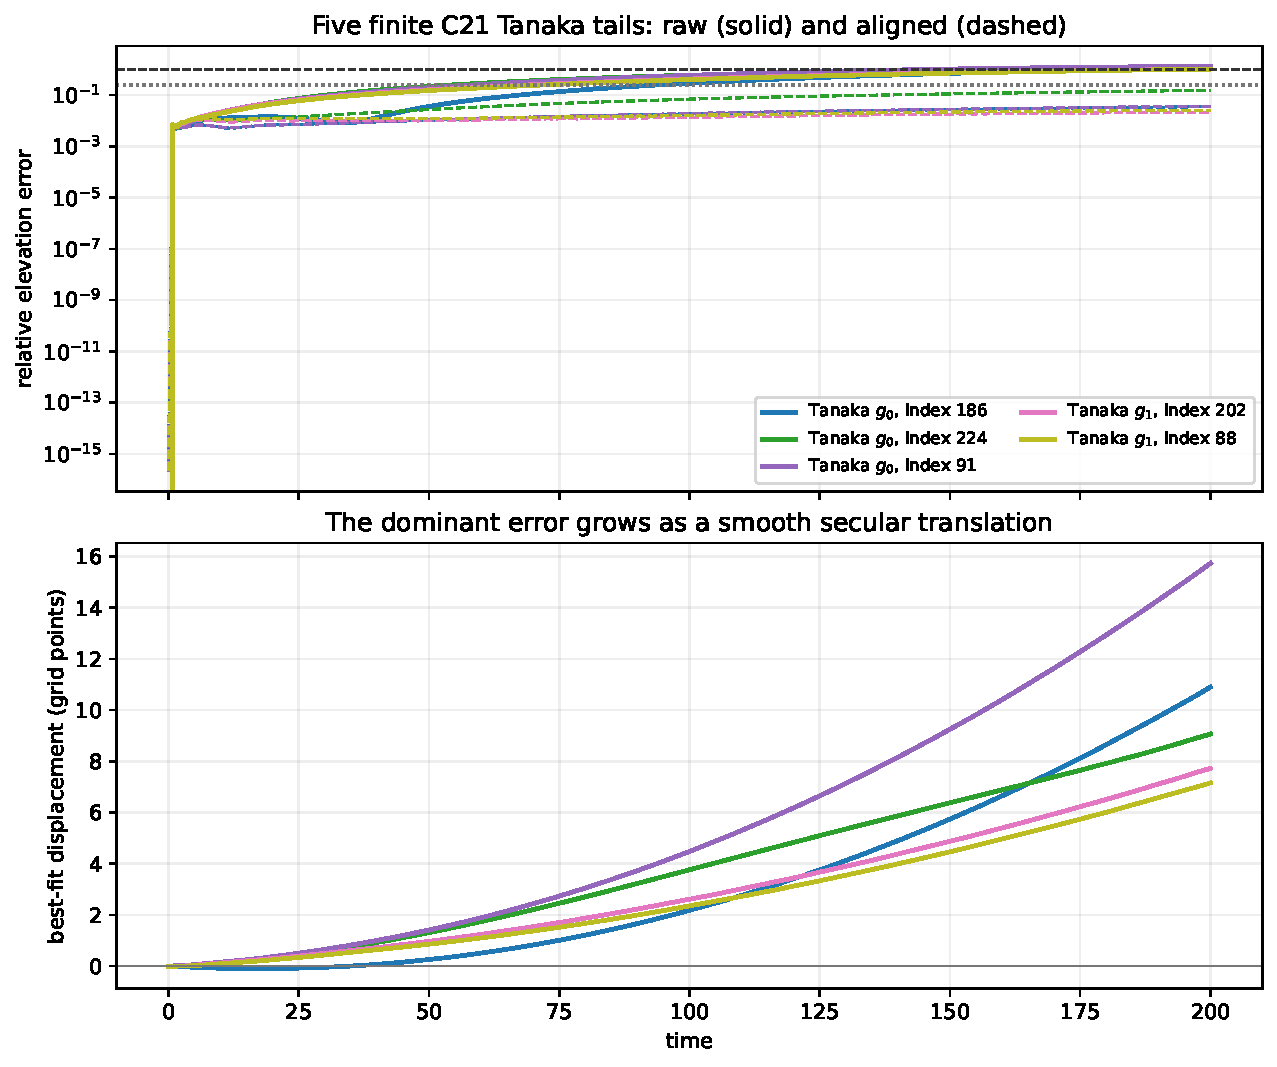
\includegraphics[width=.92\textwidth]{../figures/weekly_results_20260716/c21_worst_tanaka_error_growth.pdf}
  \caption{Raw error, error after the best translation at each saved time, and
  inferred displacement for the five C21 Tanaka cases with final raw error
  above one.}
  \label{fig:tanaka-growth}
\end{figure}

\begin{figure}[htbp]
  \centering
  \begin{subfigure}[t]{.49\textwidth}
    \centering
    
\includegraphics[width=\textwidth]{\detokenize{../figures/weekly_results_20260716/failure_frames/tanaka_g0_idx=91_case90000091_h0.018_final.png}}
    \caption{A nearly rigid displacement: raw 1.326, shifted .0368.}
  \end{subfigure}
  \hfill
  \begin{subfigure}[t]{.49\textwidth}
    \centering
    
\includegraphics[width=\textwidth]{\detokenize{../figures/weekly_results_20260716/failure_frames/tanaka_g0_idx=224_case90000224_h0.014_final.png}}
    \caption{Position plus shape/relative-crest error: raw 1.128, shifted .154.}
  \end{subfigure}
  \caption{Final order-six reference (black) and C21 prediction (red dashed)
  for two of the five large Tanaka errors.}
  \label{fig:tanaka-frames}
\end{figure}

\FloatBarrier

\subsection{Benjamin--Feir: incorrect relative modes}

The sixth raw error above one is BF-modal index 22.  Its raw error is 1.1036
and its shifted error is .8422, so one translation removes only 41.75\% of
squared error.  At modes 17, 20, and 23, the predicted-to-reference amplitude
ratios are 1.495, .305, and .968.  The shifts inferred separately from their
phase errors are $-.00699$, $+.07027$, and $-.06199$.  Since these shifts have
different signs, no single horizontal translation aligns the important modes.

\begin{figure}[htbp]
  \centering
  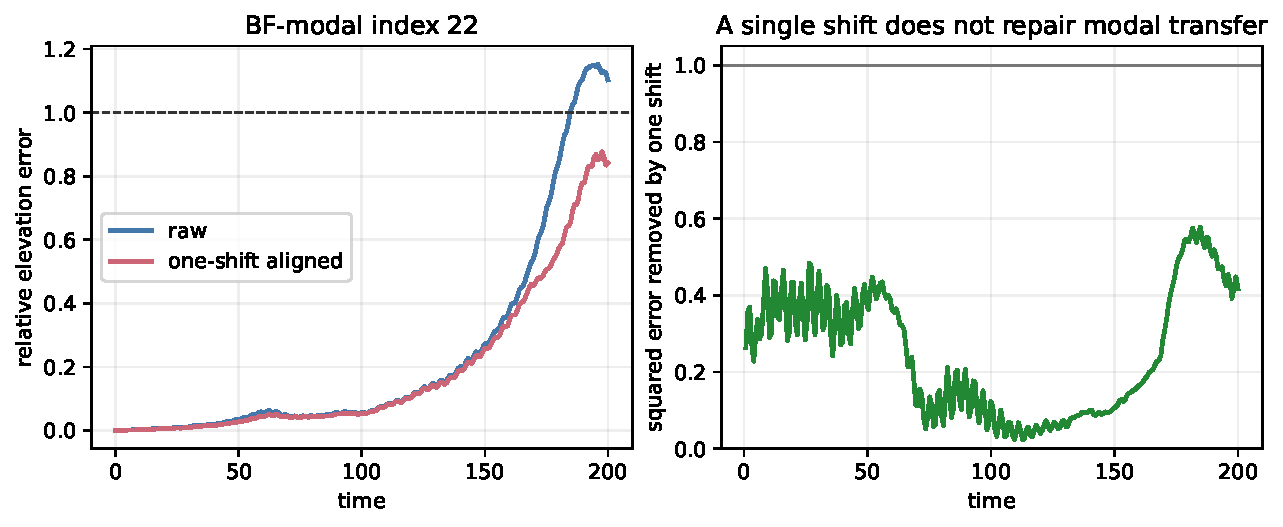
\includegraphics[width=.9\textwidth]{../figures/weekly_results_20260716/c21_worst_bf_modal_error_growth.pdf}
  \caption{Raw and shifted errors for BF-modal index 22.  The best translation
  leaves a large discrepancy because the relative mode amplitudes and phases
  are wrong.}
  \label{fig:bf-growth}
\end{figure}

\begin{figure}[htbp]
  \centering
  
\includegraphics[width=.82\textwidth]{\detokenize{../figures/weekly_results_20260716/failure_frames/bf_modal_idx=22_case94000022_h2.876_final.png}}
  \caption{Final order-six reference and C21 prediction for BF-modal index 22.}
  \label{fig:bf-frame}
\end{figure}

\FloatBarrier

\section{Why we did not add another phase-only loss}

At a model state $z$, define the complete DNO discrepancy
\begin{equation}
  d(z)=q_6(z)-q_\theta(z).
\end{equation}
We performed diagnostic rollouts that evaluated this expensive quantity at
every GL2 stage and added only a selected component to $q_\theta$.  These are
not deployable models; they ask whether one selected component is sufficient.

\begin{table}[htbp]
\centering
\small
\begin{tabular}{lrrrr}
\toprule
& \multicolumn{2}{c}{Tanaka case 24} & \multicolumn{2}{c}{Tanaka case 27} \\
Stage correction & Raw & Shifted & Raw & Shifted \\
\midrule
None (C21) & .659088 & .245457 & .336422 & .030498 \\
Fourier phase component & .625276 & .119104 & 1.024433 & .042911 \\
Local translation, width $h$ & .508067 & .225268 & 1.079470 & .043482 \\
Local translation, width $4h$ & .474397 & .151743 & .134637 & .024499 \\
Non-phase complement & .137739 & .136753 & .535542 & .027532 \\
Complete discrepancy $d$ & $2.25\times10^{-8}$ & $2.25\times10^{-8}$
& $1.94\times10^{-8}$ & $1.84\times10^{-8}$ \\
\bottomrule
\end{tabular}
\caption{Reference-assisted stage corrections.  The partial correction that
works best for case 24 is not the one that works best for case 27.}
\label{tab:corrections}
\end{table}

The complete correction makes both calculations agree with the order-six
reference to about $2\times10^{-8}$.  The defensible conclusion is limited:
none of the tested phase, local-translation, or complementary components is
sufficient for both cases.  This is why the next experiment targets the
capacity of the complete learned remainder instead of adding a fourth
phase-specific loss.

\FloatBarrier

\section{C25: the experiment currently running}

\subsection{The question}

C25 asks whether the neural approximation to the complete remainder in
\begin{equation}
  G_\theta(\eta;h)\xi
  =G_0(h)\xi+G_1(\eta;h)\xi+R_\theta(\eta,\xi,h),
  \qquad R_\theta=O(\eta^2),
  \label{eq:c25-model}
\end{equation}
was too small.  This is controlled relative to C20, not C21.  C25 does not use
C21's tangent coefficient 100; it uses C20's coefficient 10 and trains from
random initialization.

\begin{table}[htbp]
\centering
\begin{tabular}{lrr}
\toprule
Quantity & C20/C21 architecture & C25 \\
\midrule
Feature width & 512 & 640 \\
Branch rank & 256 & 320 \\
Multiplier hidden width & 128 & 160 \\
Blocks & 8 & 8 \\
Parameters & 860,928 & 1,342,400 \\
\bottomrule
\end{tabular}
\caption{The architectural change in C25.  Parameter count increases by
55.9\%.}
\label{tab:c25-size}
\end{table}

Everything else central to the test is unchanged relative to C20:
\begin{itemize}[leftmargin=*]
  \item exact $G_0+G_1$ and no analytic term beyond $G_1$;
  \item the bias-free, self-adjoint, $O(\eta^2)$ learned remainder;
  \item the complete v9 training set, batch size 1024, and learning rate
  $2\times10^{-5}$;
  \item the same loss
  \begin{equation}
    L_{H^1}+6L_{\mathrm{mode}}+10L_{\mathrm{tangent}}
    +\mathbf 1_{16\mid s}\,0.01L_{\mathrm{Hadamard}},
    \label{eq:c25-loss}
  \end{equation}
  with 500-step warmup for the mode and Hadamard coefficients.
\end{itemize}
The $\gamma^2$, finite-time, modal-phase, and Hamiltonian-conservation loss
weights are all zero.  There is no hard output cap or learned spectral cutoff.
Thus C25 has three ordinary full-batch terms and one small Hadamard term
evaluated every 16 steps; it is substantially simpler than the history needed
to motivate it.

\subsection{Status at 05:30 EDT}

Four epochs have completed.  The training log is advancing through epoch 5;
at the cutoff it had reached batch 2,197 of 5,964 (36.8\%).  The complete epochs are
\begin{table}[H]
\centering
\small
\begin{tabular}{lrrrrr}
\toprule
Epoch & Training loss & Validation loss & Validation $H^1$ & Validation mode & Validation tangent \\
\midrule
1 & .0114936 & .00969421 & .00900150 & $1.06919\times10^{-4}$ & $5.11932\times10^{-6}$ \\
2 & .00932340 & .00874953 & .00829122 & $7.22955\times10^{-5}$ & $2.45360\times10^{-6}$ \\
3 & .00867311 & .00841511 & .00801352 & $6.39104\times10^{-5}$ & $1.81328\times10^{-6}$ \\
4 & .00832224 & .00805709 & .00772591 & $5.27578\times10^{-5}$ & $1.46287\times10^{-6}$ \\
\bottomrule
\end{tabular}
\caption{C25 completed-epoch metrics at the cutoff.  All recorded values are
finite.  Expected and observed Hadamard evaluations agree in every epoch.}
\label{tab:c25-progress}
\end{table}

These are optimization measurements, not rollout results.  C25 should be
called better only if a completed checkpoint preserves zero observed
nonfinite model trajectories on valid references and improves the raw and
shifted error distributions without worsening the Benjamin--Feir or linear
panels.  The first comparison will use the fixed 64 Tanaka cases; the full
test, if warranted, is the same 256-case-per-panel evaluation used for C21.

\section{Takeaways for discussion}

\begin{enumerate}[leftmargin=*,label=\textbf{\arabic*.}]
  \item The old NaNs were preceded by an incorrect response of the learned DNO
  to small off-trajectory surface perturbations.  The Hadamard identity gave a
  direct test and training constraint for this derivative error.

  \item The C16 bundle was followed by no observed nonfinite model trajectory
  in the fixed 320-case test.  The large current errors are finite and should
  not be described as the old spectral blow-up.

  \item C21 has no observed nonfinite model trajectory among 2,508 valid new
  references.  Its median error is small, but six finite cases exceed one.

  \item Five of the six are mainly accumulated Tanaka displacement.  The
  sixth is a Benjamin--Feir relative-mode error.  These require different
  descriptions; one phase coordinate does not cover both.

  \item Exact correction of selected phase or local components does not
  improve both diagnostic Tanaka cases.  Exact correction of the complete DNO
  discrepancy does.

  \item C25 therefore tests a simple next hypothesis: enlarge the complete
  learned $O(\eta^2)$ remainder while retaining the same $G_0+G_1$
  construction and C20 loss.  Training progress is positive so far, but only
  rollout evaluation can answer the question.
\end{enumerate}

\end{document}
